\section{Numerical modeling}
This model proposes the following assumptions:
\begin{itemize}
    \item Gas is treated as an ideal gas.
    \item No Voltage loss caused by anode.
    \item The anode mass transfer process is simplified, and the anode area is merged into one anode chamber.
    \item The liquid water transferred from the GDL to the flow channel is instantaneously discharged and does not accumulate in the flow channel and anode chamber.
    \item Nitrogen does not affect the mass transfer process of hydrogen, oxygen and water, and does not affect fuel cell performance.
    \item The internal temperature of the stack is uniform, and the heat transfer process is not considered.
    \item The different cells in the stack are uniform.
\end{itemize}
In summary, the regional division and state selection of this model are shown in Figure 1. For the meanings of different variables, please refer to the symbol description.
\begin{figure}[h]
    \centering
    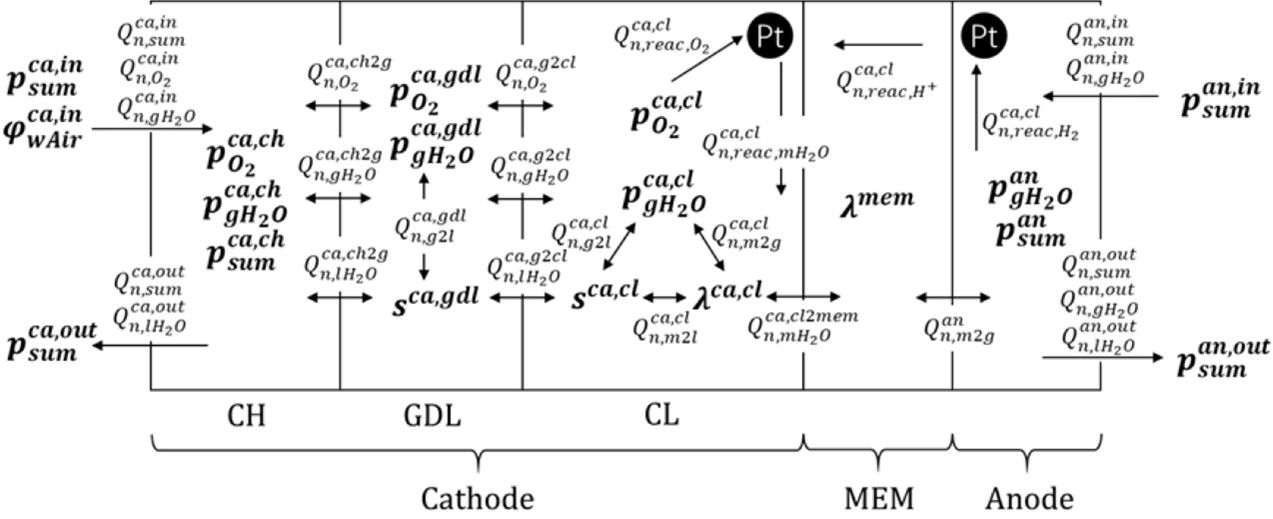
\includegraphics{Sensor_Fusion_pictures/figure1.jpg}
    \caption{Regional division and state selection of model.}
\end{figure}
\subsection{Cathode Model}
\subsubsection{Gas Transmission}

For the inlet and outlet of the channel, it can generally be simplified as nozzle to treat. When the gas is laminar flow, the inlet flow of the stack can be expressed as
\begin{equation}
    Q_{n,s u m}^{c a,i n}=k^{c a,i n}(p_{s u m}^{c a,i n}-p_{s u m}^{c a,c h})
\end{equation}

Where $Q_(n,sum)^(ca,in)$ is the total molar flow rate of the gas at the cathode inlet (kmol/s), $k^(ca,in)$ is the nozzle coefficient at the cathode inlet (kmol/kPa∙s), $p_sum^(ca,in)$ is the total pressure at the cathode inlet (kPa), and $p_sum^(ca,ch)$ is the total pressure in the cathode channel (kPa).
\par
Then the steam flow at the stack inlet can be expressed as:
\begin{equation}
    Q_{n,g H_{2}O}^{c a,i n}=Q_{n,s u m}^{c a,i n}\cdot\frac{\varphi_{w A i n}^{c a,i n} \star p_{s a t}(r^{c a,i n})}{p_{s u m}^{c a,i n}}
\end{equation}

W